\subsection{Retriever Evaluation}
\label{subsec:retriever-eval}

The retriever component plays a crucial role in the Retrieval-Augmented Generation (RAG) pipeline. It is responsible for selecting the most relevant pieces of information (chunks) from a large corpus in response to a user query. To evaluate its effectiveness, we used several well-established metrics from the information retrieval field.

\subsubsection{Evaluation Metrics}
\begin{itemize}
    \item \textbf{Mean Reciprocal Rank (MRR):}
    The MRR evaluates how highly the first relevant document appears in the ranked list of retrieved documents. For each query, the reciprocal rank is calculated as:
    
    \begin{equation*}
    \text{Reciprocal Rank} = \frac{1}{\text{rank of the first relevant document}}
    \end{equation*}
    
    Then, the MRR is the average of these reciprocal ranks across all queries:
    
    \begin{equation*}
    \text{MRR} = \frac{1}{|Q|} \sum_{i=1}^{|Q|} \frac{1}{\text{rank}_i}
    \end{equation*}
    
    A higher MRR (closer to 1) indicates that the system often retrieves the correct document in the top position, which is critical for user-facing applications.

    \item \textbf{Mean Average Precision (MAP):}
    MAP considers all relevant documents, not just the first one. For each query, it calculates the average precision across the retrieved results and then averages over all queries. It is defined as:
    
    \begin{equation*}
    \text{MAP} = \frac{1}{|Q|} \sum_{i=1}^{|Q|} \left( \frac{1}{m_i} \sum_{k=1}^{n} P(k) \cdot rel(k) \right)
    \end{equation*}
    
    Where:
    \begin{itemize}
        \item $P(k)$ is the precision at cut-off $k$
        \item $rel(k)$ is a binary indicator of relevance at position $k$
        \item $m_i$ is the total number of relevant documents for query $i$
    \end{itemize}
    
    This metric rewards systems that rank all relevant documents highly.

    \item \textbf{Recall@K (e.g., Recall@3):}
    Recall@K measures how many relevant documents are retrieved among the top K results. It is computed as:
    
    \begin{equation*}
    \text{Recall@K} = \frac{\text{\# of relevant documents in top K}}{\text{Total \# of relevant documents}}
    \end{equation*}
    \\
    In this project, we used Recall@3 since the retriever was configured to return Top-K = 3 documents. This value was chosen based on manual analysis of a dataset of FAQs and real user queries, where it was observed that most answers could be accurately supported using at most three context documents.
\end{itemize}

\subsubsection{Global MRR Benchmark Evaluation}
The dense retriever leveraging the \texttt{BGE-M3} embedding model was evaluated on a multilingual MRR benchmark dataset. The results demonstrate that \texttt{BGE-M3} consistently outperformed other embedding models across multiple languages, showcasing its strong generalization and retrieval capabilities.

The MRR scores achieved by \texttt{BGE-M3} on different languages are as follows:
\begin{itemize}
    \item English: 0.68
    \item French: 0.60
    \item Hungarian (HU): 0.64
    \item Czech (CS): 0.65
\end{itemize}

These scores highlight the model's robust ability to retrieve relevant documents effectively in various linguistic contexts, which is crucial for building a reliable AI assistant. The comparative performance is illustrated in Figure 4, which clearly shows \texttt{BGE-M3} leading other tested models on this benchmark.
\begin{figure}[htbp]
  \centering
  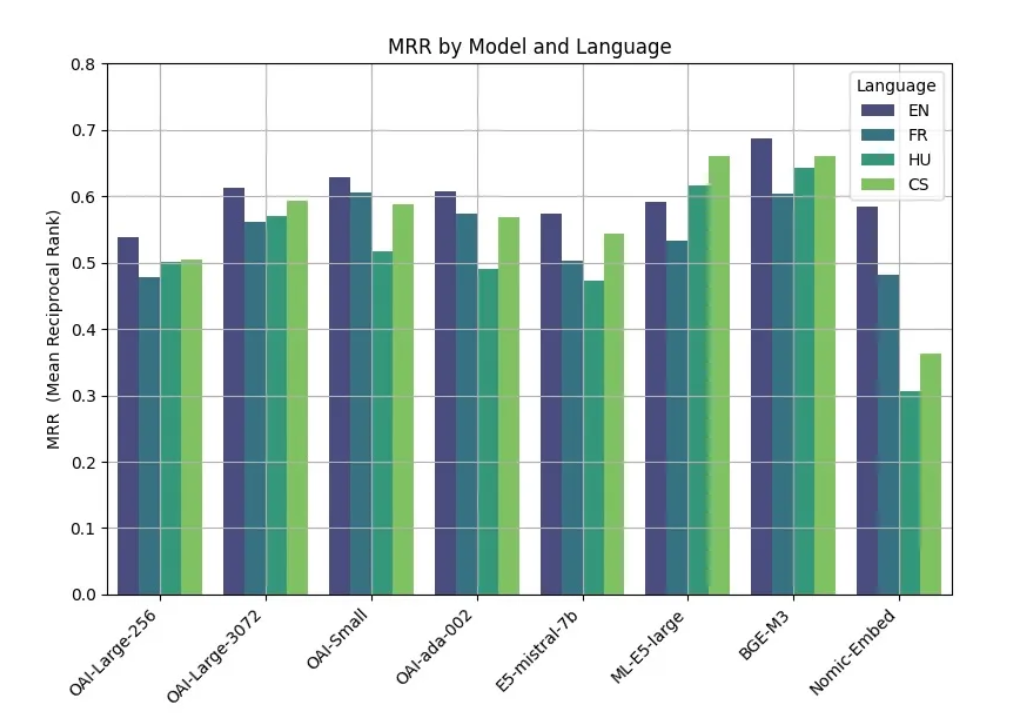
\includegraphics[width=0.8\textwidth]{rapport_pfa-main/images/MRR.png}
  \caption*{\textbf{Figure 4:} MRR Benchmark results} % Starred version
  \label{fig:indexing-process-manual}
\end{figure}


\subsubsection{Domain Evaluation}
For evaluating the retriever’s performance in the context of respiratory diseases, we created a dedicated evaluation dataset. This dataset includes approximately 50 manually selected questions related to common respiratory conditions, symptoms, and treatments. The questions were gathered from verified sources such as medical forums, FAQs, and healthcare websites to reflect real-world user inquiries. \\
We conducted a detailed manual analysis to determine which documents are relevant for answering each question. This involved reviewing the retrieved documents and annotating those essential for fully understanding the queries. This process also helped us identify the optimal number of relevant documents per question, informing retrieval parameter choices such as the top-k value. \\
This manual curation provides a high-quality ground truth for evaluation, allowing precise assessment of retriever performance in our specific domain.

\clearpage 
The retriever achieved \textbf{exceptional performance} on our respiratory disease dataset:
\vspace{0.5em}
\hrule
\begin{itemize}
    \item \textbf{Mean Reciprocal Rank (MRR):} \textbf{0.72} 
    \item \textbf{Mean Average Precision (MAP):} \textbf{0.68}
    \item \textbf{Recall@3:} \textbf{0.75}
\end{itemize}
\hrule
\vspace{0.5em}

These scores demonstrate the retriever’s effectiveness in ranking relevant documents higher, which is critical for accurate and context-aware AI assistant responses. The strong performance reflects the suitability of our embedding model and retrieval strategy tuned to the domain.\\
Nonetheless, some questions involving rare or highly specialized information showed slightly lower precision, highlighting areas for potential improvement. Overall, the results confirm that our retriever performs well in the respiratory disease domain and supports the AI assistant’s effectiveness.

\subsection{End-to-End System Evaluation}
\label{subsec:e2e-eval}

To assess the end-to-end effectiveness of our Retrieval-Augmented Generation (RAG) system, we applied the \textit{LLM-as-a-Judge} technique, where a powerful large language model evaluates generated answers using a structured rubric. Specifically, we employed \texttt{GPT-4} as an automatic evaluator to review responses generated by our system for a carefully curated set of 50 domain-specific questions.\\
As depicted in Figure 5, the evaluation pipeline feeds the user question, the RAG-generated response, and—where applicable—the baseline response into the judge model. GPT-4.0 then rates the answers on six essential dimensions, each on a scale from 0 to 10:
\begin{itemize}
    \item \textbf{Groundedness:} Alignment with retrieved context
    \item \textbf{Correctness:} Factual and domain accuracy
    \item \textbf{Coherence:} Clarity, structure, and logical flow
    \item \textbf{Relevance:} Direct response to query
    \item \textbf{Novelty:} Added value from synthesis
    \item \textbf{Overall Score:} General utility and effectiveness
\end{itemize}
\begin{figure}[htbp]
  \centering
  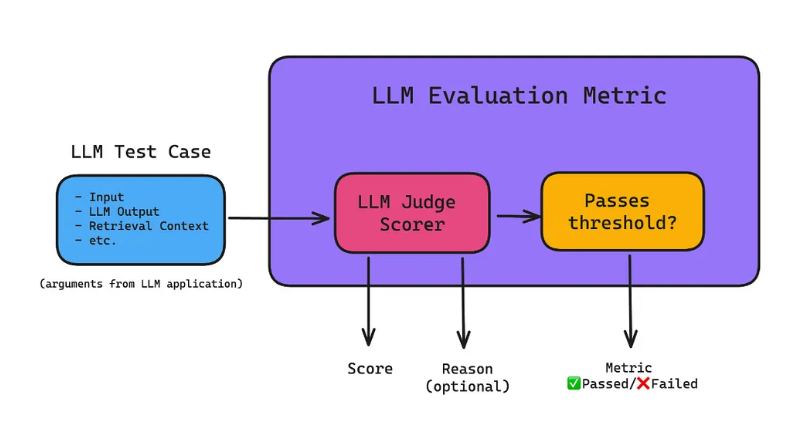
\includegraphics[width=0.8\textwidth]{rapport_pfa-main/images/LLM_AS_JUDGE.png}
  \caption*{\textbf{Figure 5:} Indexing process} % Starred version
  \label{fig:indexing-process-manual}
\end{figure}

\begin{table}[h]
    \centering
    \begin{tabular}{lcc}
        \toprule
        \textbf{Metric} & \textbf{RAG System} & \textbf{Baseline} \\
        \midrule
        Groundedness & 8.7 & 5.2 \\
        Correctness & 8.5 & 5.8 \\
        Coherence & 9.1 & 8.7 \\
        Relevance & 8.9 & 6.3 \\
        Novelty & 7.8 & 6.9 \\
        Overall Score & 8.6 & 6.4 \\
        \bottomrule
    \end{tabular}
    \caption*{\textbf{Table 1:} Performance comparison: RAG vs. Baseline (50 questions)}
    \label{tab:rag-vs-baseline}
\end{table}

To quantify the contribution of retrieval, we compared our RAG system with a baseline model that used the same Llama 3.2 1B Instruct LLM but without any contextual documents. The average scores across the 50-question evaluation set are shown in Table 1.

As observed in Table 1, the RAG system consistently outperformed the baseline across all metrics. The most substantial gains were seen in groundedness, correctness, and relevance, confirming that access to relevant, retrieved context significantly enhances the LLM’s ability to generate reliable and precise answers. While coherence remained relatively high in both cases, the RAG version improved the interpretability and factual grounding of responses, making it better suited for medical assistance applications.